\section{Task 2: Groundtrack as a Function of \texorpdfstring{$\Omega$}{Omega} and \texorpdfstring{$\omega$}{omega}}
\label{sec:task2}

The groundtrack needs the Earth-relative longitude and geocentric latitude at each $t_j$. The ECI positions in $\mathbf{R}$ are first rotated into the Earth-centered Earth-fixed (ECEF) frame $E$, which rotates about $\vect{I}_z$ at the constant rate $\Omega_e = \SI{7.2921159e-5}{\radian\per\second}$. $I$ and $E$ are aligned at $t=0$.

\begin{figure}[H]
\centering
% Redrawn from Project 2 Handwork p.5 / assignment Fig. 1 (ECI and ECEF bases, eta = Omega_e t).
\begin{tikzpicture}[>=Latex, scale=1.0, font=\small]
    \def\ang{30}
    % ECI basis
    \draw[->, thick, hwblue] (0,0) -- (3.2,0) node[right] {$\vect{I}_x$};
    \draw[->, thick, hwblue] (0,0) -- (0,3.2) node[above] {$\vect{I}_y$};
    % ECEF basis
    \draw[->, thick, hwred] (0,0) -- (\ang:3.0) node[right] {$\vect{e}_x$};
    \draw[->, thick, hwred] (0,0) -- (90+\ang:3.0) node[left] {$\vect{e}_y$};
    % common z axis (out of page)
    \draw[thick] (0,0) circle (0.12);
    \fill (0,0) circle (0.04);
    \node[below left] at (0,0) {$\vect{e}_z,\vect{I}_z$};
    % rotation angles
    \draw[->, hwgreen] (1.6,0) arc (0:\ang:1.6);
    \node[hwgreen] at (15:2.0) {$\Omega_e t$};
    \draw[->, hwgreen] (0,1.6) arc (90:90+\ang:1.6);
    \node[hwgreen] at (105:2.0) {$\Omega_e t$};
\end{tikzpicture}

\caption{ECI basis $I = \{\vect{I}_x,\vect{I}_y,\vect{I}_z\}$ and ECEF basis $E = \{\vect{e}_x,\vect{e}_y,\vect{e}_z\}$, rotated by $\eta \equiv \Omega_e t$ about $\vect{I}_z = \vect{e}_z$.}
\label{fig:t2-frames}
\end{figure}

\subsection*{Task 2-1: Transformation from ECI to ECEF}

\paragraph{(a)} From \cref{fig:t2-frames}, with $\eta = \Omega_e t$, the ECEF basis vectors in ECI components are
\begin{equation}
\vect{e}_x = \cos\eta\,\vect{I}_x + \sin\eta\,\vect{I}_y,
\qquad
\vect{e}_y = -\sin\eta\,\vect{I}_x + \cos\eta\,\vect{I}_y,
\qquad
\vect{e}_z = \vect{I}_z.
\end{equation}
Each row of $\mathbf{T}_I^E$ holds one ECEF basis vector, so that $x_e = \vect{r}\cdot\vect{e}_x$, $y_e = \vect{r}\cdot\vect{e}_y$, $z_e = \vect{r}\cdot\vect{e}_z$:
\begin{equation}
\boxed{\mathbf{T}_I^E(t) =
\begin{bmatrix} c_{xx} & c_{xy} & c_{xz} \\ c_{yx} & c_{yy} & c_{yz} \\ c_{zx} & c_{zy} & c_{zz} \end{bmatrix}
=
\begin{bmatrix} \cos(\Omega_e t) & \sin(\Omega_e t) & 0 \\ -\sin(\Omega_e t) & \cos(\Omega_e t) & 0 \\ 0 & 0 & 1 \end{bmatrix}}.
\label{eq:t2-dcm}
\end{equation}

\paragraph{(b)} \texttt{dcmI2E(t, O\_e)} returns \cref{eq:t2-dcm}, with $t$ in \si{\second} and $\Omega_e$ in \si{\radian\per\second}.

\subsection*{Task 2-2: Position in ECEF coordinates}

\texttt{eci2ecef(t\_arr, r\_arr, O\_e)} builds $\mathbf{T}_I^E(t_j)$ at each time and applies it to the matching row of $\mathbf{R}$:
\begin{equation}
\vect{r}_e(t_j) = \mathbf{T}_I^E(t_j)\,\vect{r}(t_j),
\qquad
\mathbf{R}_e = \begin{bmatrix} \vect{r}_e^T(t_0) \\ \vdots \\ \vect{r}_e^T(t_n) \end{bmatrix} \in \mathbb{R}^{(n+1)\times 3}.
\end{equation}

\subsection*{Task 2-3: Earth-relative longitude and latitude}

With $\vect{r}_e = [x_e,\,y_e,\,z_e]$ in each row of $\mathbf{R}_e$, \texttt{ecef2LonLat(R\_ecef)} evaluates, with the four-quadrant inverse tangent,
\begin{equation}
\theta_e = \tan^{-1}(y_e,\,x_e),
\qquad
\phi = \tan^{-1}\!\left(z_e,\,\sqrt{x_e^2+y_e^2}\right).
\label{eq:t2-lonlat}
\end{equation}

\subsection*{Task 2-4: Groundtrack}

The longitudes and latitudes are converted to degrees and plotted with \texttt{mercatorDisplay} (Python version of the given code)\newtxt{, with one marker per value of $\Omega$, and one figure per value of $\omega$}. \newtxt{The} track is shown over the NASA image~\cite{nasa-image} (\newtxt{\cref{fig:t2-gt90,fig:t2-gt270}}).

\begin{figure}[H]
\centering
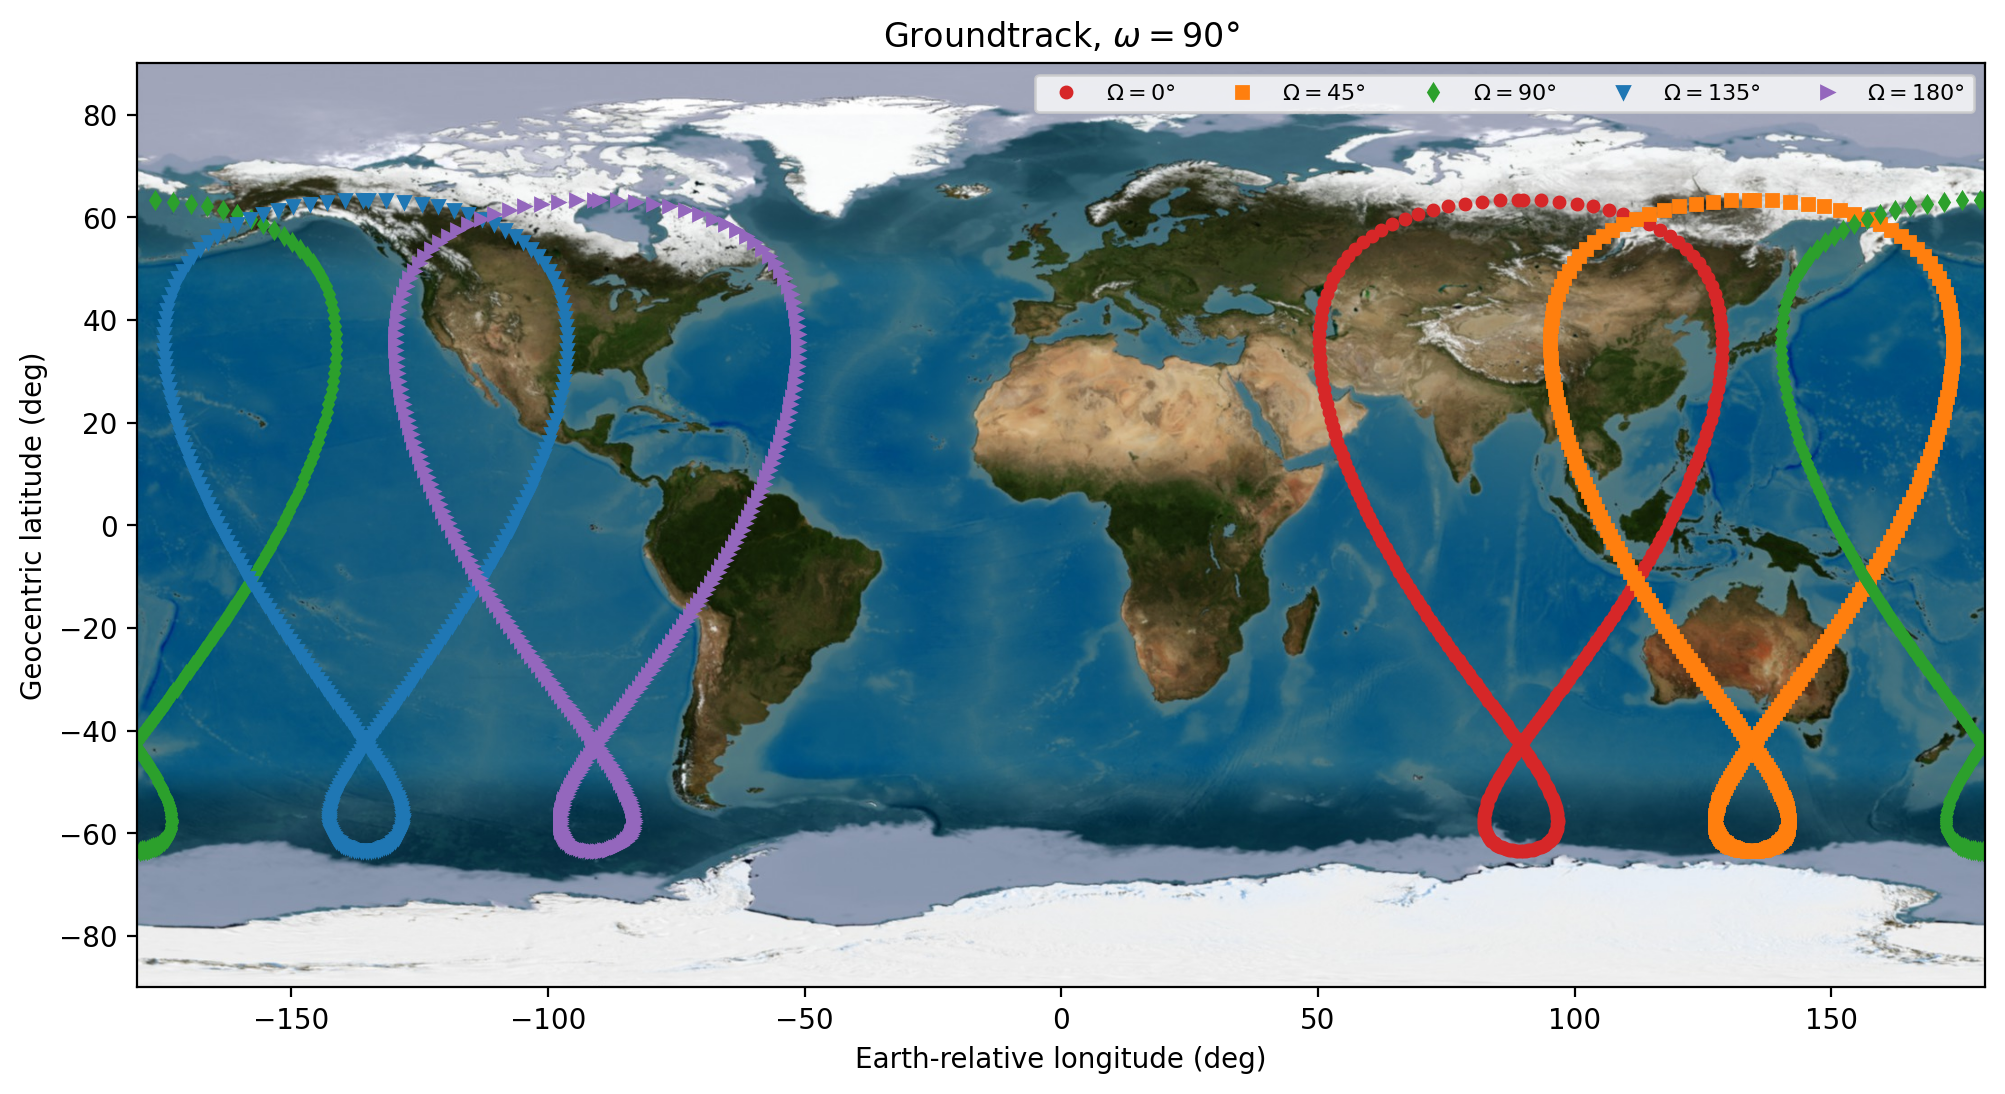
\includegraphics[width=\textwidth]{groundtrack_w90.png}
\caption{\newtxt{Groundtrack, $\omega=90^\circ$, for $\Omega=(0,45,90,135,180)^\circ$} (one marker every \SI{5}{\minute}).}
\label{fig:t2-gt90}
\end{figure}

\begin{figure}[H]
\centering
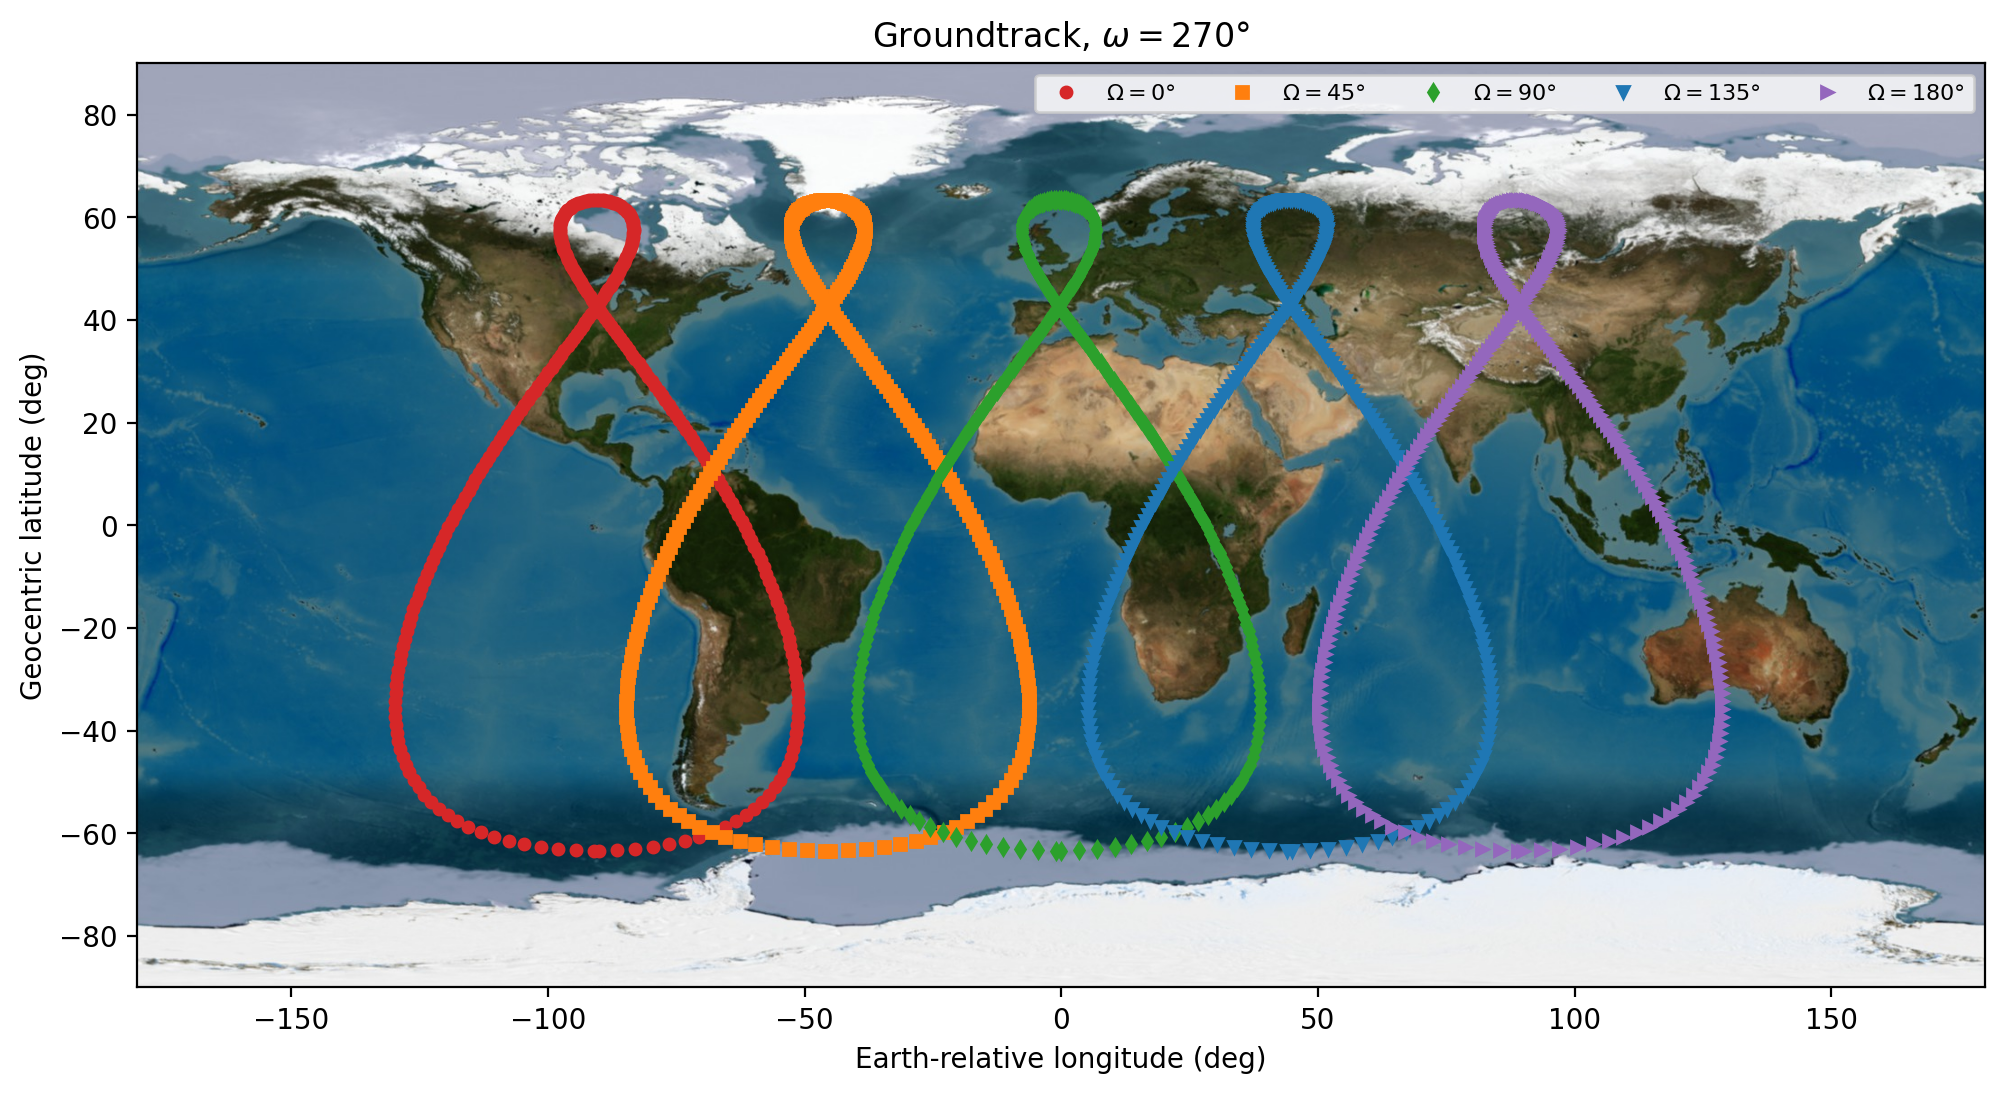
\includegraphics[width=\textwidth]{groundtrack_w270.png}
\caption{\newtxt{Groundtrack, $\omega=270^\circ$, for $\Omega=(0,45,90,135,180)^\circ$} (one marker every \SI{5}{\minute}).}
\label{fig:t2-gt270}
\end{figure}

\subsubsection*{\newtxt{Interesting feature of the groundtracks}}
\usertxt{The orbital period is $T = 24$ hours, approximately one sidereal day ($23.93$ hours). The spacecraft completes one full orbit for every rotation of the Earth, so its ground track roughly repeats in a loop, passing over the same regions at the same times. Each track looks like a figure-eight that crosses itself once, at the crossing point explained in \cref{sec:task3}. Changing $\Omega$ only shifts the track east by $\Delta\Omega$, with its shape remaining the same.}

\usertxt{Near apoapsis the spacecraft is slow and far away, tracing the small lobe of the figure-eight, and making the \SI{5}{\minute} orbit markers bunch up. Near periapsis it crosses the opposite hemisphere quickly, tracing the large lobe, and making the orbit markers appear far apart.}

\subsubsection*{\newtxt{Key difference between $\omega = 90^\circ$ and $\omega = 270^\circ$}}
\usertxt{For $\omega = 90$ deg, periapsis will always lie in the Northern hemisphere, so the apoapsis section of the figure-eight will lie in the Southern hemisphere. Since changing $\Omega$ only shifts the track east, latitudes are constant: The crossing point happens at about 43 deg, with peak apoapsis at 63.4 deg S and periapsis at 63.4 deg N. The same values are true, but in reverse for $\omega = 270$ deg (which is 180 deg apart, and thus places apoapsis in the exact opposite hemisphere).}

\FloatBarrier
